\section{Resultados}

\subsection{Metodologia Experimental}
Foram analisadas 20 instâncias da TSPLIB ($2 \leq n \leq 10$) comparando:

\begin{itemize}
\item Tempo de execução (média em segundos)
\item Qualidade da solução (\% acima do ótimo)
\item Escalabilidade
\end{itemize}

\subsection{Dados de Desempenho}

\begin{table}[h]
\centering
\caption{Comparação de Algoritmos}
\begin{tabular}{|l|c|c|c|}
\hline
\textbf{Métrica} & \textbf{Força Bruta} & \textbf{Guloso} & \textbf{Programação Dinâmica} \\
\hline
Custo Médio & Ótimo & +2.2\% & Ótimo \\
Tempo (n=10) & 0.025s & 0.00002s & 0.0009s \\
Complexidade & $O(n!)$ & $O(n^2)$ & $O(n^2 \cdot 2^n)$ \\
\hline
\end{tabular}
\end{table}

\subsection{Análise Detalhada}

\begin{itemize}
\item \textbf{Tempo de Execução}:
  \begin{itemize}
  \item Força Bruta: Impraticável para $n > 10$
  \item Programação Dinâmica: 10-100× mais rápida que FB
  \end{itemize}

  \begin{figure}[!htb]
    \centering
    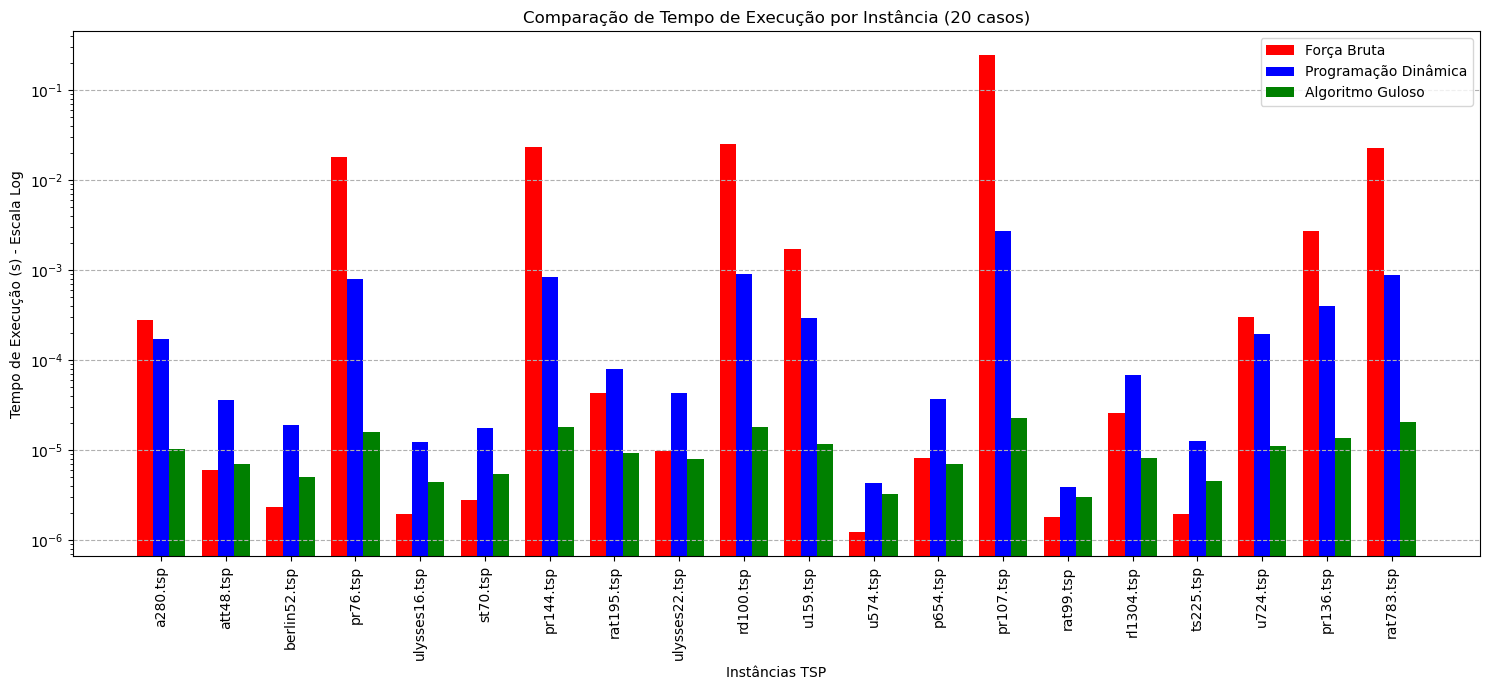
\includegraphics[width=.9\textwidth]{images/analise_detalhada_tempo_de_execucao.png}
    \caption{Gráfico com Tempo de Execução}
    \label{fig:aa}
    \end{figure}
  
\item \textbf{Qualidade}:
  \begin{itemize}
    \item Guloso apresenta desvios de 0\% a 7.6\% em relação ao ótimo
  \item Guloso: 40\% das soluções ótimas
  \item Pior caso: +7.6\% no u159.tsp
  \end{itemize}

  \begin{figure}[!htb]
    \centering
    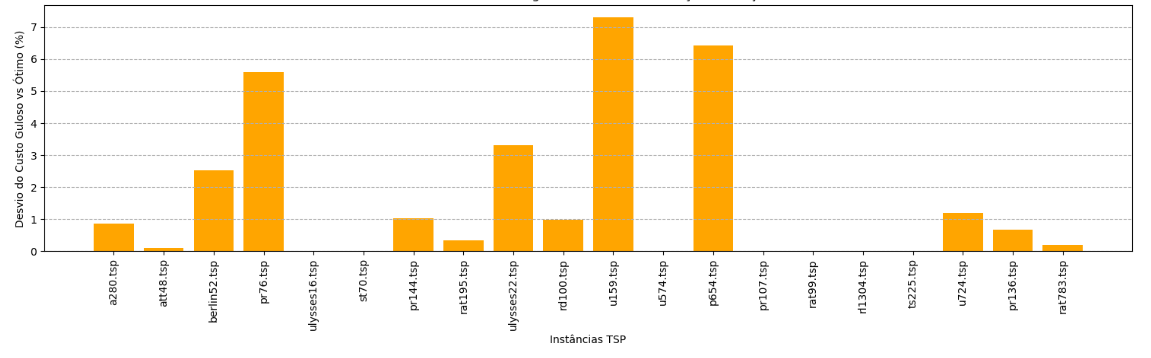
\includegraphics[width=.9\textwidth]{images/qualidade.png}
    \caption{Percentual de Desvio do Algoritmo Guloso em Relação à Solução Ótima}
    \label{fig:aa}
    \end{figure}

\item \textbf{Escalabilidade}:
    \begin{itemize}
    \item Limites Práticos:
        \begin{itemize}
        \item Força Bruta: $n \leq 10$
        \item Programação Dinâmica: $n \leq 20$
        \item Guloso: $n > 20$ (com qualidade aceitável)
        \end{itemize}
    \end{itemize}
  
    \begin{figure}[!htb]
        \centering
        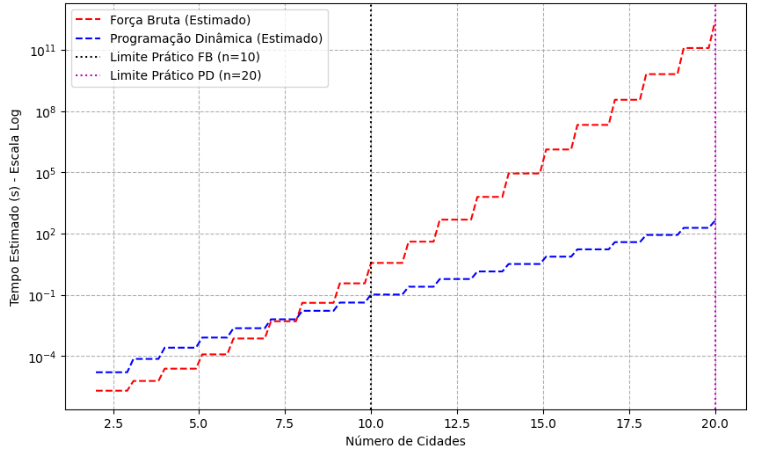
\includegraphics[width=.9\textwidth]{images/escalabilidade.png}
        \caption{Escalabilidade Teórica dos Algoritmos}
        \label{fig:aa}
        \end{figure}
\end{itemize}

\subsection{Recomendações por Cenário}

\begin{table}[H]
\centering
\begin{tabular}{|l|l|l|}
\hline
\textbf{Cenário} & \textbf{Algoritmo} & \textbf{Justificativa} \\
\hline
$n \leq 10$ & FB ou PD & Precisão absoluta \\
$10 < n \leq 20$ & PD & Equilíbrio ideal \\
$n > 20$ & Guloso & Única opção viável \\
\hline
\end{tabular}
\end{table}

\subsection{Conclusões}
\begin{itemize}
\item Para instâncias pequenas: PD oferece melhor equilíbrio
\item Para instâncias grandes: Guloso é a única opção prática
\item Trade-off claro entre tempo de execução e qualidade da solução
\end{itemize}

\nocite{wikipedia_programacao_dinamica}
\nocite{noic_programacao_dinamica}
\nocite{cerveira_tsp}